\documentclass{beamer}

\usepackage[utf8]{inputenc}
\usepackage[french]{babel}
\frenchbsetup{SmallCapsFigTabCaptions=false}
\usetheme{Boadilla} %{CambridgeUS}
\usecolortheme{default}  % default	beaver	beetle	seahorse	wolverine

\usepackage{multicol}
\usepackage[font=small,justification=justified]{caption}

\usepackage[natbib,backend=biber,style=ieee,language=french]{biblatex}
\DefineBibliographyExtras{french}{\renewcommand{\mkbibnamefamily}[1]{{\hyphenrules{nohyphenation}#1}}}

%%%%%%%%% MAAAAATHS

\usepackage{cool}
\usepackage{upgreek}
\usepackage{upref}
\usepackage{mathtools}
\usepackage{amsmath}
\usepackage{amsfonts}
\usepackage{amsthm}
\theoremstyle{definition}
\usepackage{amssymb}
\usepackage[scaled=1.]{rsfso}
\usepackage[scaled=1.,mathscr]{urwchancal}
\usepackage{stmaryrd}

\newcommand{\RR}{\ensuremath{\mathbb{R}}}
\newcommand{\Zseq}[2]{\ensuremath{\left\{#1 , \dots, #2\right\}}}
\newcommand{\interffZ}[2]{\ensuremath{\left\llbracket#1 , #2\right\rrbracket}}
\newcommand{\interfoZ}[2]{\ensuremath{\left\llbracket#1 , #2\right\llbracket}}
\newcommand{\interofZ}[2]{\ensuremath{\left\rrbracket#1 , #2\right\rrbracket}}
\newcommand{\interooZ}[2]{\ensuremath{\left\rrbracket#1 , #2\right\llbracket}}
\newcommand{\interff}[2]{\ensuremath{\left[#1 , #2\right]}}
\newcommand{\interfo}[2]{\ensuremath{\left[#1 , #2\right[}}
\newcommand{\interof}[2]{\ensuremath{\left]#1 , #2\right]}}
\newcommand{\interoo}[2]{\ensuremath{\left]#1 , #2\right[}}

%%%%%%%%%

\newcommand{\Cad}{C'est-à-dire}
\newcommand{\cad}{c'est-à-dire}

\title[\textit{The group fused Lasso}]{\textit{The group fused Lasso for multiple change-point detection}}
\subtitle{Une implémentation en Python 3}
\author[A. Huat, J. Lefevre]{Alexandre Huat\inst{1}, Joseph Lefevre\inst{1}}
\institute[INSA Rouen]{\inst{1}Institut National des Sciences Appliquées de Rouen\\Dépt. Architecture des Systèmes d'Information}
\date{\today}
\addbibresource{gfl_references.bib}
% \logo{\includegraphics[height=2em]{logo-vekia.png}}



\begin{document}
	\maketitle

\section{Introduction}			
	\begin{frame}{\insertsection}
		\begin{block}{Objectif}
			Détecter des points de changement dans des signaux multidimensionnels.
		\end{block}
	
		\begin{block}{Référence}
			\nocite{*}
%			\begin{otherlanguage}{english}
			\printbibliography[title=none]
%			\end{otherlanguage}
		\end{block}	
	\end{frame}

\section{Détection de points de changement}			
\begin{frame}{\insertsection}
	\begin{block}{La méthode vue en cours}
		CUSUM. 
	\end{block}

    \begin{block}{Propriété de cette méthode de CPD (changepoint detection)}
    	Hors-ligne, non-supervisé, pas d'informations à priori nécessaires. 
    \end{block}

    \begin{block}{De nombreuses autres méthodes existent}
    	SST (Singular Spectrum Transformation), KCD (kernel change detection). 
    \end{block}
\end{frame}

\section{Formulation}
	\begin{frame}[allowframebreaks]{\insertsection}
		\begin{block}{Variation totale convexe}
			Soit $Y\in\RR^{n\times p}$ un signal multidimensionnel. Détecter des points de ruptures dans $Y$ consiste à trouver $U\in\RR^{n\times p}$ la meilleure approximation de $Y$ qui contient le moins de ruptures. Soit résoudre :
			\begin{equation}
				\label{eq:TV}
				\min_{U\in\RR^{n\times p}} \frac{1}{2} \lVert Y - U \rVert^2 + \lambda \sum_{i=1}^{n-1}\frac{\lVert U_{i+1,\bullet} - U_{i,\bullet} \rVert^2}{d_i}
			\end{equation}	
			avec $\lambda \in \RR^+$ un coefficient de régularisation du nombre de ruptures et $(d_i)_{i \in \Zseq{1}{n-1}}$ des poids positionnels. Le schéma de poids idéal est :
			\begin{equation}
				d_i=\sqrt{\frac{n}{i(n-i)}}
			\end{equation}
		\end{block}
		Les points de plus forte variation totale de $U$ sont alors considérés comme les points de ruptures de $Y$.
			 
		\begin{block}{Reformulation : \textit{The group fused Lasso}}
			On pose $\beta \in \RR^{(n-1) \times p}$ tel que :
			\begin{equation}
				\beta_{i, \bullet} = \frac{\lVert U_{i+1,\bullet} - U_{i,\bullet} \rVert^2}{d_i}
			\end{equation}
			
			Puis, par changement de variables, on montre que \eqref{eq:TV} équivaut à :
			\begin{equation}
				\min_{\beta \in \RR^{(n-1) \times p}} \frac{1}{2} \lVert \bar{Y} - \bar{X} \beta \rVert^2 + \lambda \sum_{i=1}^{n-1} \lVert \beta_{i, \bullet} \rVert^2
			\end{equation}
			où $\bar{Y} \in \RR^{n \times p}$ est le signal centré et $\bar{X} \in \RR^{n \times (n-1)}$ est $X$ centrée avec $X$ une matrice triangulaire strictement inférieure telle que $\forall i>j, X_{i,j}=d_j$.
		\end{block}
	
		
	\end{frame}

\section{Résolution}
	\begin{frame}[allowframebreaks]{\insertsection}
		\begin{block}{Algorithmes}
			\citet{gfl} proposent deux algorithmes de résolution :
			\begin{enumerate}
				\item Par descente de gradient par bloc de coordonnées ; ce qui donne une solution exacte.
				\item Par \textit{least-angle regression} (LARS) ; ce qui donne une solution approchée mais converge plus rapidement.
			\end{enumerate}
		\end{block}
	
		\begin{block}{Implémentations}
			\begin{enumerate}
				\item $<100$ lignes de code
				\item not working yet...
			\end{enumerate}
		\end{block}
	\end{frame}

\section{Résultats}
	\begin{frame}[allowframebreaks]{\insertsection}
		\begin{figure}
			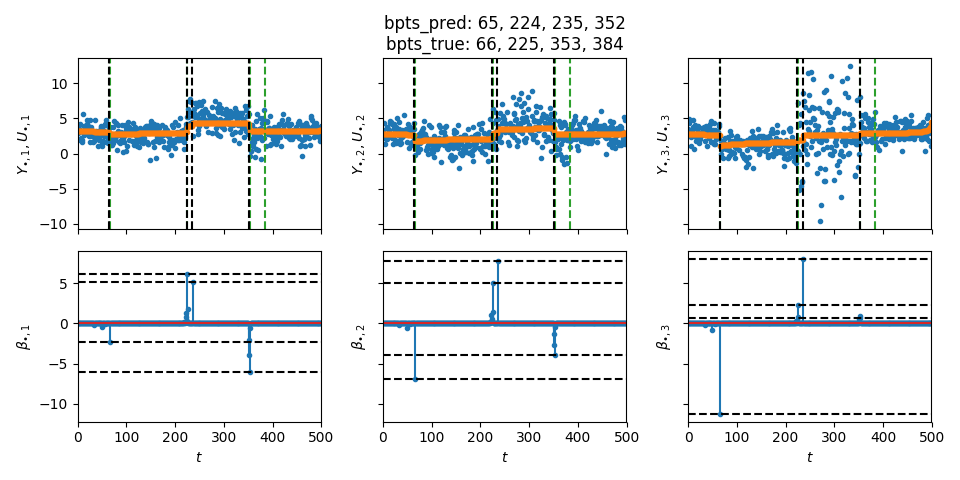
\includegraphics[width=1\textwidth]{algo1simu.png}
			\caption{Résultats de l'algorithme 1 avec un signal simulé en trois dimensions. Les points de rupture sont les mêmes pour chaque sous-signal mais les bruits gaussiens qui leurs sont appliqués sont différents.}
			\label{fig:algo1simu}
		\end{figure}
	
		\begin{figure}
%			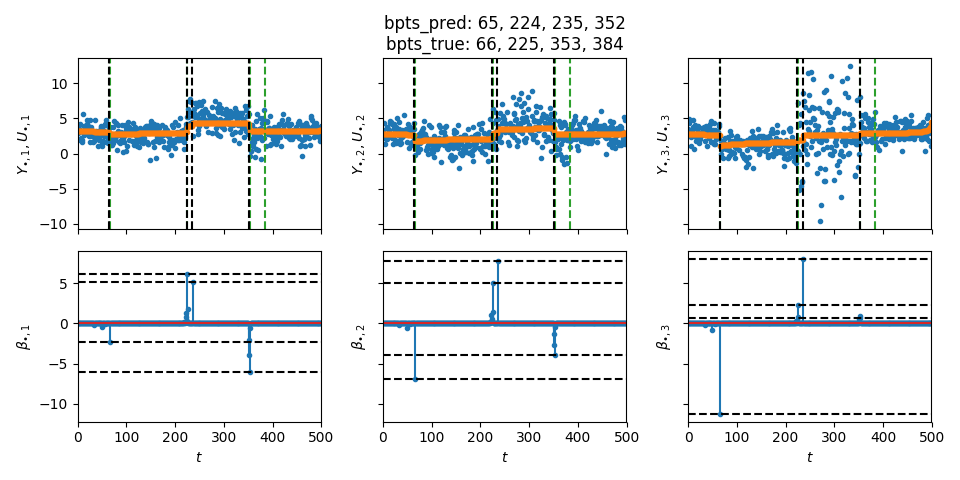
\includegraphics[width=1\textwidth]{algo1simu.png}
			\caption{Résultats de l'algorithme 1 avec un signal réel ………………}
			\label{fig:algo1real}
		\end{figure}
	\end{frame}

\section{LARS}
\begin{frame}[allowframebreaks]{\insertsection}
	\begin{block}{Principe}
		Rechercher le bon paramètre lambda et avoir une hiérarchie des points de changement.
	\end{block}
	
	\begin{figure}
		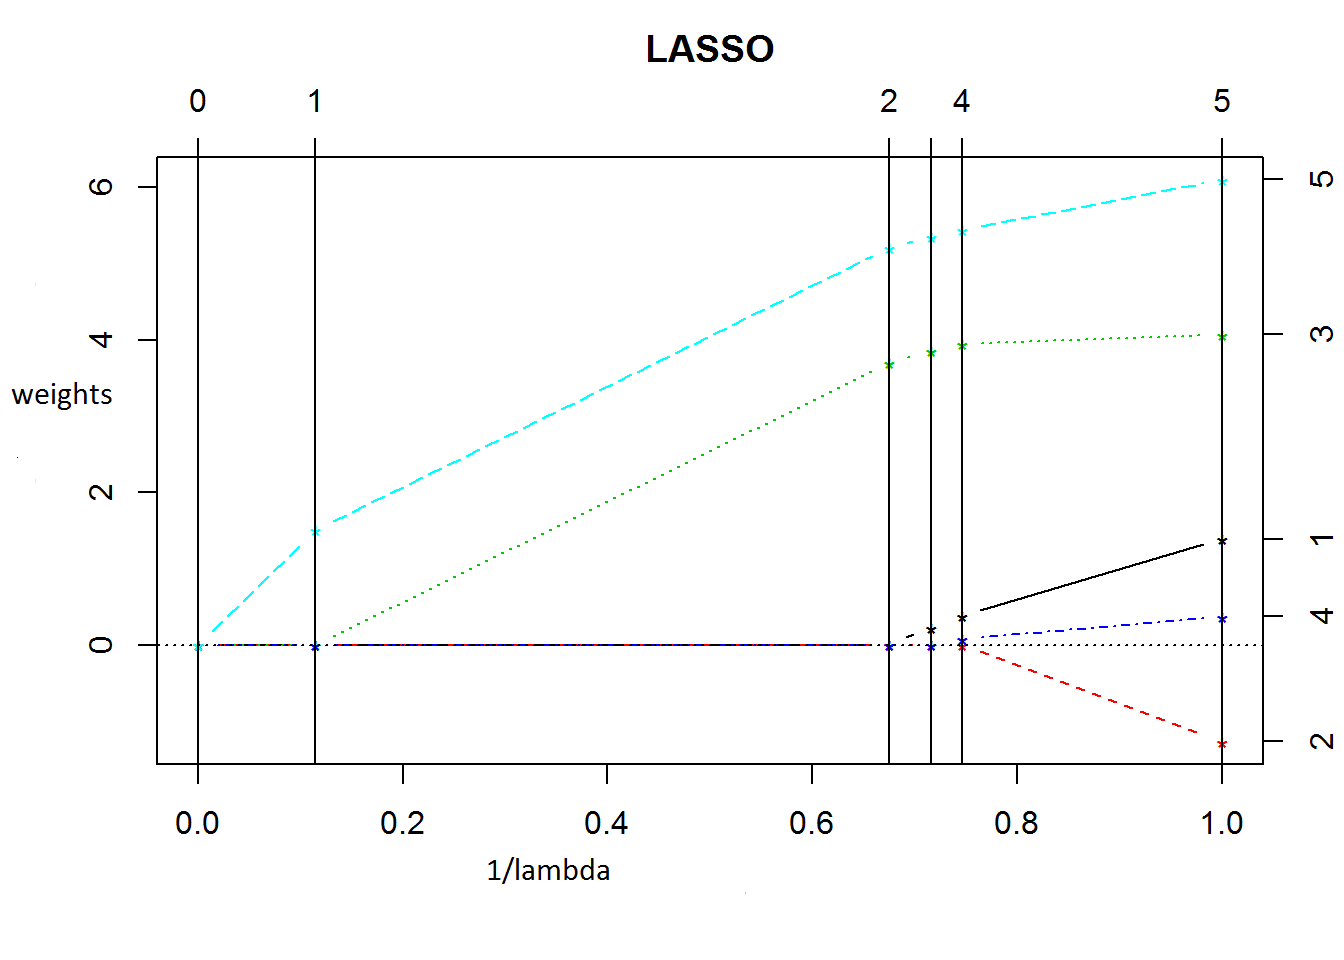
\includegraphics[scale=0.35]{lars.png}
		\caption{Représentation graphique de la sortie d'un LARS.}
		\label{fig:lars}
	\end{figure}
\end{frame}

\section{Applications}
\begin{frame}[allowframebreaks]{\insertsection}
	\begin{block}{Principe}
		\begin{enumerate}
			\item Reconnaissance vocale - Segmentation des mots, de phrases, etc. ;
			\item Monitoring de conditions médicales d'un patient (détection de sortie de coma, etc.) ;
			\item Détection de changement de climat ;
			\item Détection de changement de morceaux dans un album (pour intégrer une pub entre deux morceaux).
		\end{enumerate}
	\end{block}
	
\end{frame}

\end{document}
